\section{Sample Spaces}

\begin{definition}
An experiment is any process that can be repeated with a well-defined set of outcomes. Example: roll a die, toss a coin.
\end{definition}

\textbf{Sets:} discrete/finite, discrete/infinite, continuous

\begin{definition}
A sample space is the set of all possible outcomes of an experiment. Example: $S = \{1, 2, 3, 4, 5, 6\}$, $S = \{H, T\}$
\end{definition}

\begin{definition}
The union of $A$ and $B$, $A \cup B$, is all elements in $A$ or $B$.
\end{definition}

\begin{definition}
The intersection of $A$ and $B$, $A \cap B$, is all elements in both $A$ and $B$.
\end{definition}

\begin{definition}
$A$ and $B$ are mutually exclusive (disjoint) if $A \cap B = \emptyset$.
\end{definition}

\begin{definition}
The complement of $A$, $A^c$, is the set of elements not in $A$: $S - A$.
\end{definition}

\section{Probability}

\begin{definition}
The function $P$ is a probability function if it satisfies:
\begin{enumerate}
\item $P(A) \in [0, 1]$ for all $A \subseteq S$
\item $P(S) = 1$
\item If $A$ and $B$ are disjoint, then $P(A \cup B) = P(A) + P(B)$
\item If $A_1, A_2, \ldots$ are disjoint, then $P\left(\bigcup_{i=1}^{\infty} A_i\right) = \sum_{i=1}^{\infty} P(A_i)$
\end{enumerate}
\end{definition}

\begin{lemma}
$P(A^c) = 1 - P(A)$
\end{lemma}

\textbf{Proof:} $A \cup A^c = S$, $A \cap A^c = \emptyset$, so $P(S) = P(A \cup A^c) = P(A) + P(A^c) = 1$. Therefore, $P(A^c) = 1 - P(A)$.

\subsection{Fair Dice Example}
If we roll a fair die, $P(i) = \frac{1}{6}$ for $i = 1, 2, \ldots, 6$.

$P(\{1, 2\} \cup \{3, 4\} \cup \{5, 6\}) = P(\{1\}) + P(\{2\}) + \cdots + P(\{6\}) = 6 \cdot P(\{1\}) \Rightarrow P(\{1\}) = \frac{1}{6}$

Note: If all elements in $S$ are equally likely, $P(A) = \frac{\text{\# in } A}{\text{\# in } S}$

\subsection{Card Example}
Roll a fair dice, find $P(\text{sum} = 5)$.

\begin{center}
\begin{tabular}{c|cccc}
 & $A$ & $B$ & Total \\
\hline
 & 1 & 4 & 5 \\
 & 2 & 3 & 5 \\
 & 3 & 2 & 5 \\
 & 4 & 1 & 5
\end{tabular}
\end{center}

There are 26 people, find $P(\text{at least 2 same birthday})$.

$1 - P(\text{0 different})$

\begin{lemma}[Addition Rule]
$P(A \cup B) = P(A) + P(B) - P(A \cap B)$
\end{lemma}

If disjoint: $P(A \cup B) = P(A) + P(B) - 0 = P(A) + P(B)$

Proof: $P(A \cup B^c) + P(A \cap B^c) + P(B \cap A^c) = P(A \cup B)$

\textbf{Prove:} If $A \subseteq B$, then $P(A) \leq P(B)$

If $A \subseteq B$, $B^c \cap A = \emptyset$

$B = A \cup (A^c \cap B)$ (disjoint union), so $P(B) = P(A) + P(A^c \cap B)$

Because $P(\cdot)$ is non-negative, $P(B) \geq P(A)$

\section{Counting}

\subsection{Example 2.8}
Given $A, B, C$:
\begin{enumerate}
\item[a)] none occur: $A^c \cap B^c \cap C^c$ (only $A$ occurs: $A \cap B^c \cap C^c$)
\item[b)] all three occur: $A \cap B \cap C$ (exactly one occurs: $(A \cap B^c \cap C^c) \cup (A^c \cap B \cap C^c) \cup (A^c \cap B^c \cap C)$)
\item[c)] at least one occurs: $A \cup B \cup C$ ($(A^c \cap B \cap C) \cup (A \cap B^c \cap C)$)
\end{enumerate}

$P(A) = 0.3$, $P(B) = 0.7$, $P(A \cap B) = 0.1$, WANTED

$P(A \cup B) = 0.3 + 0.7 - P(A \cap B) = 0.9 - 0.5 = 0.4$

Blue/green/red

$P(A \cup B) = 0.5 + 0.7 = P(A \cap B) = 0.9$

$P(A \cap B) = 0.3$

\begin{center}
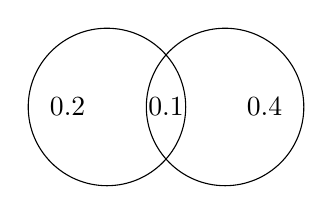
\begin{tikzpicture}
\draw (0,0) circle (1cm);
\draw (1.5,0) circle (1cm);
\node at (-0.5,0) {0.2};
\node at (2,0) {0.4};
\node at (0.75,0) {0.1};
\end{tikzpicture}
\end{center}

\subsection{Counting Example}
Choose a card at random: $P(A) = \frac{3}{7}$, $P(A \cap \text{red}) = \frac{15}{70} = \frac{3}{14}$, $P(A \cup \text{red}) = \frac{4}{7}$

Choose two at random without replacement (conditional probability): if the first card has an $A$, find $P(\text{second} = A) = \frac{2}{69}$, $P(\{2^{\text{nd}} = A\} \mid \{1^{\text{st}} = A\}) = \frac{1}{51} = \frac{1}{17}$

One card: $P(\text{red} \mid A) = \frac{15}{30} = 0.5$

$P(\text{red} \mid A) = \frac{P(\text{red} \cap A)}{P(A)} = \frac{3/7}{1} = \frac{3}{7}$

\section{Conditional Probability}

\begin{definition}
$P(A \mid B) = \frac{P(A \cap B)}{P(B)}$
\end{definition}

Choose two without replacement: $P(\text{both blue}) = P(\{1^{\text{st}} \text{ blue} \cap 2^{\text{nd}} \text{ blue}\}) = P(\text{blue})P(2^{\text{nd}} \text{ blue} \mid 1^{\text{st}} \text{ blue})$

$= \frac{14}{70} \cdot \frac{13}{69} = \frac{182}{4830} = \frac{14}{70} = \frac{1}{5}$

Choose 5 without replacement: $P(\text{at least one is blue}) = 1 - P(\text{no blue}) = 1 - \frac{56 \cdot 55 \cdots}{70 \cdot 69 \cdots}$

Example: Two buckets - 11 blue/1 green, 2 blue/3 green. Choose one from bucket one and move to bucket 2, choose 1 from bucket 2:

$P(1^{\text{st}} \text{ blue} \cap 2^{\text{nd}} \text{ blue}) = \text{WORK}$

$P(1^{\text{st}} \text{ green} \cap 2^{\text{nd}} \text{ blue}) = \frac{1}{4}$

$P(2^{\text{nd}} \text{ blue}) = \frac{6}{12}$

\subsection{Total Probability - Given Events}
Total probability: Given $A_1, A_2, \ldots, A_n$ with $A_i \cap A_j = \emptyset$ ($i \neq j$) and $\bigcup A_i = S$,

then $P(B) = \sum_{i=1}^n P(B \cap A_i) = \sum_{i=1}^n P(A_i)P(B \mid A_i)$
